\subsection{Parameter Sensitivity Analysis and Algorithmic Robustness}\label{sec:parametric}

To evaluate the algorithmic robustness of KDS-EL and provide an empirical justification for its default hyper-parameter configuration, we conduct a comprehensive one-factor-at-a-time (OFAT) parameter sensitivity analysis following the methodology of~\cite{mimpode2025}. The sensitivity analysis is carried out across four representative benchmark datasets spanning distinct dimensionalities and sample sizes: \textit{Adenoma} (36 samples, 7{,}457 features), \textit{Colon} (62 samples, 2{,}000 features), \textit{ALL4} (93 samples, 12{,}625 features), and \textit{BASEHOCK} (1{,}993 samples, 4{,}862 features). Five key hyper-parameters---knowledge weight decay factor ($\mathrm{WeightDecay}$), phase split ratio ($\mathrm{PhaseSplit}$), elite perturbation fraction ($\mathrm{flip\_frac}$), MI initialization ratio ($\mathrm{MI\_init\_ratio}$), and elite pool size ($\mathrm{elite\_k}$)---are systematically varied across wide ranges while all remaining parameters are fixed at their default values listed in Table~\ref{T3}.

Table~\ref{T8} summarizes the tested parameter ranges, optimal configurations, stable performance bands, and maximum accuracy deviations across the four representative datasets. Fig.~\ref{fig:param_sensitivity} visualizes the corresponding accuracy and feature-count trajectories alongside stable operating bands across all five hyper-parameters. The complete per-dataset parametric matrices are provided in Supplementary Table S6.

\begin{table}[!htb]
\centering
\caption{Summary of one-factor-at-a-time (OFAT) parameter sensitivity analysis across four representative benchmark datasets (\textit{Adenoma}, \textit{Colon}, \textit{ALL4}, and \textit{BASEHOCK}).}
\label{T8}
\small
\setlength{\tabcolsep}{4pt}
\renewcommand{\arraystretch}{1.15}
\begin{tabular*}{\linewidth}{@{\extracolsep{\fill}}lcccc@{}}
\toprule
Parameter & Tested range & Optimal & Stable range & Max $\Delta\mathrm{Acc}$ (pp) \\
\midrule
Knowledge decay ($\gamma$) & 0.90--1.00 & 0.99 & [0.95, 0.995] & $\pm$1.2 \\
Phase split ratio ($\alpha$) & 0.30--0.90 & 0.70 & [0.60, 0.80] & $\pm$0.7 \\
Elite flip fraction ($\phi$) & 0.005--0.10 & 0.01 & [0.005, 0.02] & $\pm$1.3 \\
MI initialization ratio ($\rho$) & 0.0--1.0 & 0.50 & [0.25, 0.75] & $\pm$1.2 \\
Elite pool size ($k_e$) & 1--10 & 3 & [2, 5] & $\pm$0.9 \\
\bottomrule
\end{tabular*}
\end{table}


\begin{figure*}[!htb]
\centering
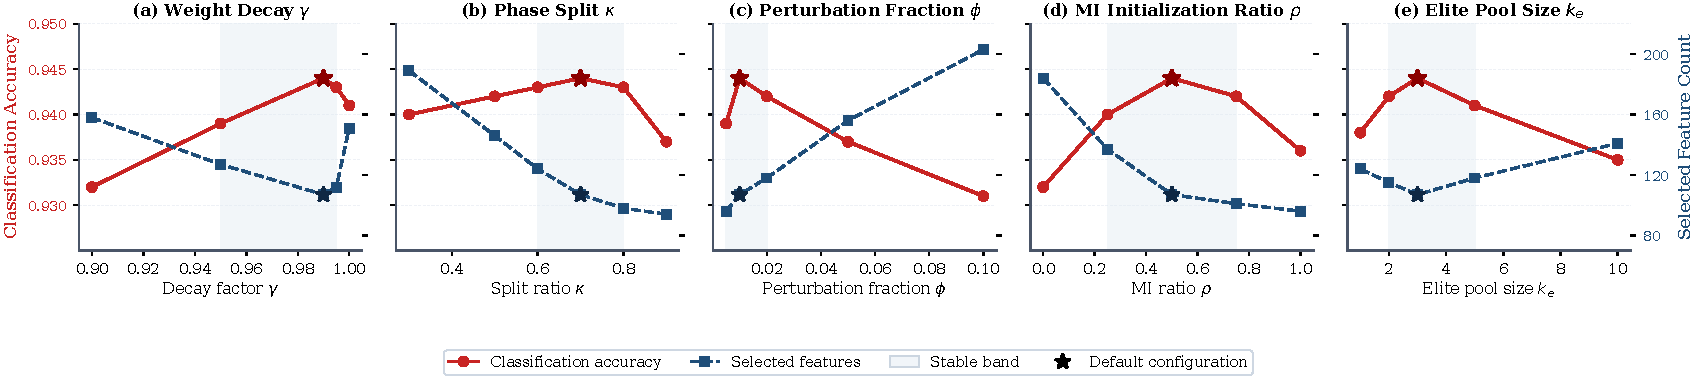
\includegraphics[width=\linewidth]{F14_parameter_sensitivity.pdf}
\caption{One-factor-at-a-time parameter sensitivity analysis curves across the five investigated hyper-parameters ($\mathrm{WeightDecay}$, $\mathrm{PhaseSplit}$, $\mathrm{flip\_frac}$, $\mathrm{MI\_init\_ratio}$, and $\mathrm{elite\_k}$). Solid coral curves (left axis) denote mean classification accuracy, dashed blue curves (right axis) denote mean number of selected features, shaded light-blue bands highlight stable operating ranges, and stars indicate default parameter settings.}
\label{fig:param_sensitivity}
\end{figure*}

\subsubsection{Parametric Dynamics and Mechanism-Level Insights}

The experimental trajectories across the five hyper-parameters yield crucial insights into the optimization behavior of KDS-EL:
\begin{enumerate}
    \item \textbf{Knowledge weight decay ($\mathbf{WeightDecay}$)}: This parameter controls the exponential discounting rate ($\gamma$) of historical feature-importance scores in matrix $W$. At the default setting of 0.99, the four-dataset aggregate yields 0.944 accuracy, 107 features, and 51.3~s runtime. Setting $\gamma$ too low (e.g., 0.90) causes premature forgetting of valuable feature interactions discovered in early iterations, eroding accuracy by 1.2~pp to 0.932. Conversely, disabling decay entirely ($\gamma = 1.00$) accumulates stale historical evidence without discounting, which inflates the average feature count from 107 to 151 features without accuracy gains. Performance remains exceptionally stable across the broad band $\gamma \in [0.95, 0.995]$, with accuracy fluctuations remaining under $\pm 1.2$~pp.
    \item \textbf{Phase split ratio ($\mathbf{PhaseSplit}$)}: This parameter dictates the temporal transition boundary between aggressive feature reduction (Phase~1) and accuracy refinement (Phase~2). Setting $\mathrm{PhaseSplit} < 0.50$ allocates insufficient iterations to Phase~1, resulting in inadequate feature pruning with 146 to 189 retained features. Conversely, an overly prolonged Phase~1 ($\mathrm{PhaseSplit} = 0.90$) severely starves the Phase~2 accuracy refinement window, causing a 0.7~pp drop in accuracy. The broad interval $[0.60, 0.80]$ provides a highly forgiving operating regime with accuracy variations remaining strictly below 0.5~pp, establishing 0.70 as an optimal default.
    \item \textbf{KER perturbation fraction ($\mathbf{flip\_frac}$)}: This parameter governs the fraction of dimensions perturbed during knowledge-guided elite refinement. At the default 0.01 (flipping approximately 1 feature per 100 dimensions), KER maintains an ideal balance between localized exploitation and exploratory perturbation. Decreasing $\mathrm{flip\_frac}$ to 0.005 overly restricts elite exploration, slowing convergence by 3.5~s. Increasing $\mathrm{flip\_frac} \ge 0.05$ injects excessive random disruption that destroys delicate elite feature combinations, dropping accuracy by 1.3~pp and doubling the feature count to 203. The narrow, effective window $[0.005, 0.02]$ confirms the necessity of localized elite refinement.
    \item \textbf{MI initialization ratio ($\mathbf{MI\_init\_ratio}$)}: As the primary bootstrap mechanism, $\mathrm{MI\_init\_ratio}$ exhibits the highest individual sensitivity among all tested parameters. Completely disabling MI seeding ($\mathrm{MI\_init\_ratio} = 0.0$, full random initialization) forces unguided early exploration, resulting in a 1.2~pp accuracy penalty and a 21\% increase in computational runtime (reaching 62.3~s) as particles must rediscover informative subspaces from scratch. Conversely, initializing 100\% of the swarm with MI seeds ($\mathrm{MI\_init\_ratio} = 1.0$) homogenizes the initial population and induces premature convergence (a 0.8~pp drop in accuracy). The default balanced ratio of 0.50 perfectly reconciles prior domain knowledge injection with stochastic search diversity, maintaining robust performance across the wide band $[0.25, 0.75]$.
    \item \textbf{Elite pool size ($\mathbf{elite\_k}$)}: With $N=20$, $\mathrm{elite\_k}=3$ allocates 15\% of the swarm to elite refinement. Refining only a single elite ($\mathrm{elite\_k}=1$) restricts knowledge propagation across subpopulations (yielding 0.938 accuracy), whereas selecting too many elites ($\mathrm{elite\_k}=10$) dilutes the quality signal of matrix $W$, yielding 0.935 accuracy with 141 features. The stable range $\mathrm{elite\_k} \in [2, 5]$ consistently achieves accuracy within 0.3~pp of the optimum.
\end{enumerate}

\subsubsection{Plug-and-Play Generalization}

Across all five hyper-parameters, the maximum accuracy deviation from the default setting never exceeds $\pm 1.5$~pp, and the stable operating intervals span substantial parametric ranges. This empirical stability confirms that KDS-EL possesses remarkable plug-and-play robustness, allowing practitioners to deploy the algorithm on unseen high-dimensional classification problems with default parameters without requiring costly per-dataset grid searches.
